\section{\index{Thermal models}}
There are three options for thermal simulation in \simname; 1) A constant temperature through the device. This is recommended for most simulation and is set at 300K by default; 2) a lattice thermal solver \ref{sec:lattice}, this solves the heat equation throughout the device taking into account self heating.  This is useful for simulating devices which get hot through their operation; 3) A hydrodynamic thermal \ref{sec:energy} solver which does not assume the electron, hole and lattice temperatures are equal.  This is useful for simulating heat flow over heterojunctions or where carriers do not have time to relax to the lattice temperature.

The drift diffusion equations given in \ref{eq:ndrive} and \ref{eq:pdrive} are only valid in isothermal conditions.  The full transport equations as derived from the BTE \cite{Azoff} are given by

\begin{equation}
\label{eq:Jnfull}
 \textbf{J}_n = \mu_e n \nabla E_c +\frac{2}{3} \mu_e n \nabla \bar{W} + \frac{2}{3} \bar{W} \mu_e \nabla n - \mu_e n \bar{W} \frac{\nabla m^*_e}{m^*_e}
\end{equation}


\begin{equation}
\label{eq:Jpfull}
 \textbf{J}_p = \mu_h p \nabla E_v -\frac{2}{3} \mu_h p \nabla \bar{W} - \frac{2}{3} \bar{W} \mu_h \nabla p + \mu_p p \bar{W} \frac{\nabla m^*_h}{m^*_h}
\end{equation}

where $\bar{W}$ is the average kinetic energy of the free carriers as given by \ref{eq:energy}.  If the average energy is assumed to be 3/2kT, \ref{eq:Jnfull} and \ref{eq:Jpfull}, return to the standard drift diffusion equations. Note the full form of these equations is required when not using MB statistics.

The thermal model can be configured in the thermal ribbon \ref{fig:thermal}. Usually the thermal model is turned off and a constant temperature (300K) is assumed across the device. If you wish to adjust this temperature click on the "Set temperature icon".  The thermal model can be turned on by clicking on the candle to the on the far left of the thermal ribbon, so that a flame appears.  Various heating sources can be enabled or disabled by depressing the buttons to the right of the ribbon. Boundary conditions can be set in the "Boundary Conditions" window, thermal constants of the material layers can be changed in the "Thermal parameters window".

\begin{figure}[ht!]
\centering
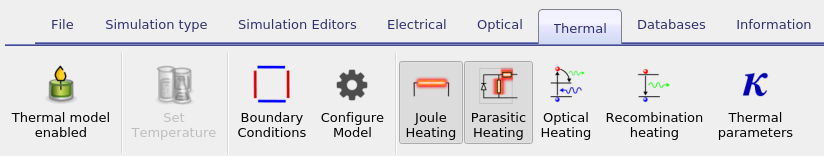
\includegraphics[width=120mm]{./images/thermal_ribbon.png}
\caption{Thermal}
\label{fig:thermal}
\end{figure}

\subsection{Lattice thermal model}
\label{sec:lattice}

When solving only the lattice heat equation heat transfer and generation is given by

\begin{equation}
0 = \nabla   \kappa_{l} \nabla T_{L} +H_j +H_r +H_{optical}+H_{shunt}
\end{equation}

where joule heating ($H_j$) is give by

\begin{equation}
H_j= J_{n} \frac{\nabla E_{c}}{q} + J_{h} \frac{\nabla E_{h}}{q} ,
\end{equation}

recombination heating ($H_r$) is given by, 
\begin{equation}
H_r=R(E_{c}-E_{v})
\end{equation}

optical absorption heating is given by,

\begin{equation}
H_{optical}
\end{equation}

and heating due to the shunt resistance is given by 
\begin{equation}
H_{shunt}=\frac{J_{shunt} V_{applied}}{d}.
\end{equation}

The thickness of the device is given by d. Note shunt heating is only in there to conserve energy conservation.



\subsection{Energy balance - hydrodynamic transport model}
\label{sec:energy}
If you turn on the electrical and hole thermal model, then the heat source term will be replaced by

\begin{equation}
H=\frac{3 k_{b}}{2} \Bigg ( n (\frac{T_{n}-T_{l}}{\tau_{e}}) + p (\frac{T_{p}-T_{l}}{\tau_{h}})\Bigg) +R(E_{c}-E_{v})
\end{equation}

and the energy transport equation for electrons

\begin{equation}
S_n=-\kappa_n \frac{dT_{n}}{dx}-\frac{5}{2} \frac{k_{b}T_{n}}{q} J_{n}
\end{equation}

and holes,

\begin{equation}
S_p=-\kappa_p \frac{dT_{p}}{dx}+\frac{5}{2} \frac{k_{b}T_{p}}{q} J_{p}
\end{equation}

will be solved.

The energy balance equations will also be solved for electrons,

\begin{equation}
\frac{dS_{n}}{dx}=\frac{1}{q}\frac{dE_{c}}{dx} J_{n}-\frac{3 k_{b}}{2} \Bigg( R T_{n}+ n(\frac{T_{n}-T_{l}}{\tau_{e}}) \Bigg)
\end{equation}

and for holes

\begin{equation}
\frac{dS_{p}}{dx}=\frac{1}{q}\frac{dE_{v}}{dx} J_{p}-\frac{3 k_{b}}{2} \Bigg( R T_{p}+ n(\frac{T_{p}-T_{l}}{\tau_{e}}) \Bigg)
\end{equation}

The thermal conductivity of the electron gas is given by

\begin{equation}
\kappa_{n}=\Bigg ( \frac{5}{2} +c_n\Bigg) \frac{{k_{b}}^2}{q} T_{n} \mu_n n
\end{equation}

and for holes as,

\begin{equation}
\kappa_{p}=\Bigg ( \frac{5}{2} +c_p\Bigg) \frac{{k_{b}}^2}{q} T_{p} \mu_p p
\end{equation}



\newpage
